\section{Evaluation} 
\label{sec:evaluation}

We empirically explore AutoMon's performance on several functions of increasing complexity, using both real-world and synthetic data.
In particular, we investigate:
\begin{enumerate}[leftmargin=*]
    \item The tradeoff between communication and approximation error.
    \item Scalability in vector length, runtime, and the number of nodes.
    \item The effectiveness of our neighborhood-size tuning procedure.
    \item The impact of AutoMon's features on the communication cost and accuracy: ADCD local constraints, slack, and lazy sync.
    \item Communication and bandwidth on a real-world WAN.
\end{enumerate}


Our main performance metrics are communication and error.
For communication, we focus on the number of messages sent during an experiment.\footnotemark{} 
Since AutoMon is designed to keep $f(\bar{x})$ between $L$ and $U$, we also measure the maximum error $\vert f(x_0)-f(\bar{x}) \vert$.

\footnotetext{
Though we include bandwidth measurements in \S\ref{sec:distributed-experiment},
we focus on message count for several reasons.
First, we are comparing algorithms, not systems.
The number of messages is a common metric for comparing distributed algorithms because it is independent of any particular network setup and the underlying messaging stack, and because different functions and datasets have different dimensions~\cite{2021_icde_distance_lemma}. 
The size of our payload is fixed and small; given the details above, inferring bandwidth is straightforward.
Second, AutoMon is fully compatible with sketching techniques for reducing message size (see \S\ref{sec:related_work}).
Moreover, there is existing work on reducing the bandwidth of GM-based methods~\cite{2021_icde_distance_lemma,samoladas2019functional}; we leave their implementation for future work.
Lastly, in some settings, the number of messages can be more important than the bandwidth due to the power consumed by turning on the wireless radio~\cite{anastasi2009energy,Stylianopoulos2018gmsystems}.
}

We implemented the prototype in Python.
It uses JAX~\cite{jax2018github} 0.2.1 for automatic differentiation (AD) to compute the Hessian and an L-BFGS-B solver from SciPy~\cite{2020SciPy_NMeth} 1.6.2 to find the extreme eigenvalues.

\subsection{Experimental Setup}

The input for each experiment is the source code for a function $f$ and a dataset comprised of $n$ data streams, one for each node in the system.
The nodes maintain a sliding window over the data stream, and the local vector is defined as the average of the last $W$ samples in the window.
We emphasize that nothing in AutoMon requires a sliding window; it is concerned only with the local vector $x$.

We use discrete event simulation to simulate the distributed network on a single machine.
Most experiments simulate a network of fixed-rate sensors:
in each simulation round, every node reads a data update from its local stream, updates its local vector, and runs the AutoMon node code.
For DNN intrusion detection experiments, only one node reads new data in each round of simulation, using the timestamps encoded in the dataset.
During the experiment, we collect statistics about the messages that are sent between the nodes and the coordinator, the approximation error, missed violations, and so on.
%
In all the experiments, we use AutoMon with Algorithm~\ref{algo:sub_domain_tuning} for neighborhood-size tuning, lazy sync with LRU, and slack.
Unless stated otherwise, we use 10 nodes for the synthetic datasets.

We compare AutoMon with several baseline approaches:

\begin{itemize}[noitemsep, leftmargin=*]
\item \textbf{Centralization:} Every node sends its local vector after every update.
For many distributed functional monitoring tasks, including those that can use sketches, centralization is state-of-the-art since local changes require sending updated sketches~\cite{2021_icde_distance_lemma}.

\item \textbf{Periodic:} Every node sends its local vector once every $P$ simulation rounds (or $P$ time units), where $P$ is a period parameter.
This approach is easy to reason about, but is not adaptive.
It therefore suffers from many missed violations when the period is out of sync with the changes in the data.


\item \textbf{CB:} Convex Bound~\cite{lazerson:lightweight_monitoring} is a state-of-the-art GM-based approach.
For functions with a CB local constraint~\cite{lazerson:lightweight_monitoring}, we include CB in our experiments. 
We run it with lazy sync and slack.

\end{itemize}


\subsection{Functions and Datasets} 
\label{sub_sec:functions_and_datasets}

\begin{figure}
	\centering
	{\label{sub_fig:function_values_and_error_bound_around_it}
	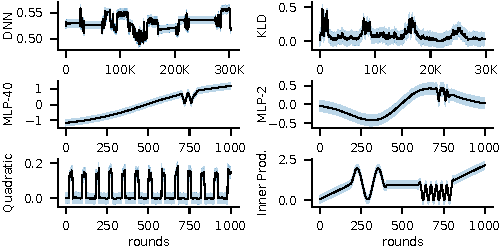
\includegraphics[width=1.0\columnwidth]{figures/function_values_and_error_bound_around_it.pdf}}
	\caption{
	    The functions and datasets used in evaluation.
	    Lines show function value for the default dimension over time;
		shaded area shows approximation bounds $\pm \epsilon$.
	}
	\label{fig:function_value_and_error_bound_around_it}
\end{figure}

We monitor different functions and use different datasets: synthetic for exploring the impact of different parameters on AutoMon and real-world, to evaluate AutoMon's performance over real data.
For synthetic datasets, we used 200 rounds for neighborhood-size tuning data and run the experiment for 1000 rounds.
For real data, the number of rounds is determined by the size of the dataset and we used $\sim 1.5\%$ of the data for tuning.
We now describe the functions that we use and the dataset for each function.
Figure~\ref{fig:function_value_and_error_bound_around_it} shows the value of each function during a run, as well as the additive error bound.
For synthetic datasets, we use the default dimensions, number of nodes, and error bound.

\begin{figure*}
	\centering
	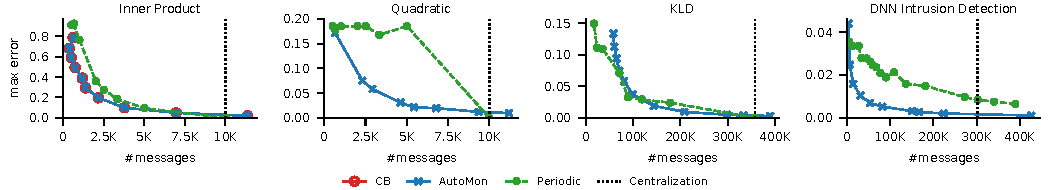
\includegraphics[width=\textwidth]{figures/max_error_vs_communication.pdf}
	\caption{
		Error-communication tradeoff when monitoring different functions with several algorithms;
		lower and to the left is better.
		Each point represents the total number of messages (X axis) and maximum error (Y axis) in one monitoring run, with a specific setting of approximation error bound (or period, for Periodic).
	}
	\label{fig:error_communication_tradeoff}
\end{figure*}

\begin{itemize}[noitemsep, leftmargin=*]


\item \textbf{MLP-}$\bm{d}$\textbf{:}
a neural network with an input layer of dimension $d$, three fully-connected hidden layers with $\tanh$ activation function, and a single output neuron with no special activation (identity function).
The function is therefore:
\begin{align*}
    f(x) =
    W_4 \cdot \varphi \left( W_3 \cdot \varphi \left( W_2 \cdot \varphi \left( W_1 \cdot x  + b_1  \right) + b_2  \right) + b_3 \right) + b_4 \text{~,}
\end{align*}
where $W_i$ and $b_i$ are the respective weights and biases of the hidden layers, and $\varphi$ is the $\tanh$ activation function, applied element-wise.
We trained these weights to evaluate the function  $x_1 \exp \left( - \frac{1}{d-1} \sum_{i=1}^{d}x_i^2 \right)$, and monitor the output of the trained network $f(\bar{x})$.
%
We use a synthetic dataset with $x_1$ sampled from the normal distribution $\mathcal{N}(\mu, 0.1^2)$ with the mean $\mu$ starting at $-2$ and increasing gradually over time.
$x_2, ..., x_d$ are sampled from $\mathcal{N}(2, 0.1^2)$ for half the nodes, and we use $\mathcal{N}(-2, 0.1^2)$ for the remaining nodes.
The data contains some outlier samples:
the mean value of $x_1$ changes to 0 for 20 rounds starting from round 720, and then again from round 760.
The default dimension $d$ in our experiments is 40.






\item \textbf{DNN for Intrusion Detection:}
a deep neural network for intrusion detection, based on the KDDCup-99 dataset~\cite{kddcup99}.
Each sample in the dataset represents a single network connection.
The samples consist of 41 features and are labeled as either normal or an attack.
For this classification task, we used a DNN with 5 fully-connected hidden layers comprising 512, 64, 32, 16, and 8 neurons in each layer, respectively, all using the ReLU activation function.
The output layer contains a single neuron with sigmoid activation.
After using the ``10\% KDD'' dataset to train the network, the trained network achieved 0.933 accuracy, 0.98 precision, and 0.93 recall on the ``Corrected KDD'' test set~\cite{kayacik2005selecting}.

We use the ``Corrected KDD'' test set as the data stream, resulting in a stream of 311029 samples.
%
We divided the data into 9 local streams according to the application-type feature of the data.
For applications that had many samples, we used a round-robin approach for load balancing and divided the samples between multiple nodes: ``ECR\_i'' was divided between 5 nodes and ``Private'' was divided between 2 nodes.
Another single node was responsible for all ``Http'' samples, and the last node was responsible for the other 62 applications.



\item \textbf{KLD:}
The Kullback–Leibler divergence function for discrete probability distributions $P$ and $Q$,
defined on the same probability space $\Omega$: $D_{KL}(P \| Q) = \sum_{\omega \in \Omega} P(\omega) \log \left( P(\omega) / Q(\omega) \right).$

We use a real-world air pollutant dataset~\cite{air_quality_dataset} collected hourly from $n=12$ air-quality monitoring sites in Beijing over 4 years (34,536 data records per site).
For each node (i.e., site), we used the PM10 attribute as $P$ and the PM2.5 attribute as $Q$.
Both attribute values are between 0 and 500, and we divided this range into $d/2$ bins, resulting in a local vector $x=[p,q]$, where $p,q \in \mathbb{R}^{d/2}$ are the local probability vectors for PM10 and PM2.5, respectively;
we use a sliding window of size $W=200$; 
in each round we update $p$ and $q$ with the new measurements.

Since KLD is undefined when $Q$ contains zero entries, we use a common variant which adds a small constant value $\tau$ to the entries of $p$ and $q$ before computing the function
$ f(x)=f([p, q]) = \sum_{i=1}^{d/2} p_i \log \left( p_i / q_i \right)$.
We use $\tau = 1 / \left( n W \right)$, the minimal possible value of the probability vectors in this setting.
Since $f$ is convex, AutoMon's approximation error is guaranteed.

We control the dimension of the function by changing the number of bins $d/2$.
By default, $d=20$.

\item \textbf{Inner Product:}
$f(x)=f([u,v]) = \langle u, v\rangle$, with a synthetic dataset that contains quiet phases as well as rapid changes in the data.
We generated the vectors $u, v \in \mathbb{R}^{d/2}$ such that $f([u,v])$ is a combination of a monotonic increasing function, a sine wave with low and high frequency, and a monotonic constant function.
We control the dimension of the function by changing the dimension of $u$ and $v$.
By default, $d=40$.

\item \textbf{Quadratic Form:}
$f(x) = x^T Q x$, where $Q \in \mathbb{R}^{dxd}$ is a random matrix with entries drawn from a standard normal distribution.
AutoMon uses ADCD-E for this function since its Hessian is constant.
We use synthetic data with each entry of $x \in \mathbb{R}^d$ sampled from the normal distribution $\mathcal{N} (0, 0.1^2)$.
A single ``outlier'' node gets an alternating pattern: 40 samples drawn from $\mathcal{N} (0, 0.1^2)$ followed by 40 samples drawn from $\mathcal{N} (-10, 0.1^2)$.
We use $d=40$.

\end{itemize}



For KLD, the node receives the frequency vector of the samples in the sliding window and the sliding window size is 200 samples.
For the other functions, the node receives the average vector of the samples in the sliding window and the sliding window size is 20 samples.
We start updating the nodes with data only after all the sliding windows of all the nodes are full.




\subsection{Error-Communication Tradeoff} \label{sub_sec:error_communication_tradeoff}
There is an inherent tradeoff between the approximation error and the resulting communication.
A communication-efficient algorithm should use minimal communication and produce a low error.




We compare AutoMon with the baselines for four functions, two with synthetic and two with real-world datasets.
In each run, we monitor the functions using a different approximation error bounds (or period values for Periodic), count the total number of messages and the maximum approximation error, and plot the resulting tradeoff curve.
The best algorithm is the one that achieves the lowest error and communication.
Figure~\ref{fig:error_communication_tradeoff} shows the tradeoff curves of AutoMon and the different baselines.

AutoMon exhibits the best tradeoff overall.
It produces a low error at a fraction of the number of messages needed by Centralization.
It also uses fewer or a similar amount of messages to those required by the non-adaptive Periodic algorithm.

\betterparagraph{Inner Product}
AutoMon automatically achieves identical performance to the carefully tailored CB-based approach of Lazerson et al.~\cite{lazerson:lightweight_monitoring}.
The CB-based algorithm uses the following identity to represent the inner product as a difference between two convex functions: $\langle x,y \rangle = \frac{1}{4}\norm{x+y}^2 - \frac{1}{4}\norm{x-y}^2$.
This form is equivalent to ADCD-E (due to space limitation, the proof is omitted).
While~\cite{lazerson:lightweight_monitoring} provides a CD representation for a specific functions, AutoMon automatically finds such a representation for any function.

\betterparagraph{Quadratic Form}
This function's value can change rapidly, as shown in Figure~\ref{fig:function_value_and_error_bound_around_it}.
The only way to obtain a small approximation error with Periodic is to have a period of 1 (i.e., Centralization); any larger period will result in high approximation errors.
In contrast, AutoMon is adaptive and can provide a smooth, superior, tradeoff between communication and efficiency.

\betterparagraph{KLD}
AutoMon yields a tradeoff that is similar to the Periodic algorithm, but with a smoother, better-controlled tradeoff curve.
Recall however, that the Periodic algorithm is non-adaptive, and the curves in Figure~\ref{fig:error_communication_tradeoff} are derived post-hoc.
Conversely, AutoMon is adaptive and can handle changes in the data distribution.
Moreover, as described above, AutoMon provides a deterministic guarantee for KLD, unlike the Periodic algorithm.

\betterparagraph{DNN}
AutoMon sends fewer messages than Periodic across all $\epsilon$ values.
Unlike the other datasets where local data for all nodes updates every round, the DNN dataset only updates a single node at a time.
This means the function changes gradually, which AutoMon exploits, while the non-adaptive Periodic sends updates from all nodes once per period even when changes are small.
Moreover, since the period parameter now represents a time interval (number of rounds) rather than the number of data samples, Centralization uses fewer messages than Periodic with a period of 1.

\begin{figure}
	\centering
	{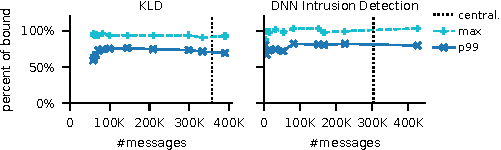
\includegraphics[width=1.0\columnwidth]{figures/percent_error_kld_and_dnn.pdf}}
	\caption{
	    AutoMon communication and error for KLD and DNN.
	    Max (dashed) and 99th percentile (solid) error are shown as percentage of the requested approximation bound.
	    }

	\label{fig:percent_error_kld_and_dnn}
\end{figure}

\betterparagraph{Error Relative to Bound}
Figure~\ref{fig:percent_error_kld_and_dnn} shows AutoMon's relative error with respect to the error bound $\epsilon$ for KLD, where AutoMon guarantees the approximation accuracy (\S\ref{sec:correctness_guarantees}), and for DNN, where there is no such guarantee.
Despite the lack of guarantee, DNN's error profile is similar to KLD:
In practice AutoMon's error is below the approximation bound 99\% of the time for both functions.
Even in the rare cases for DNN when the maximum error is above the bound, it is still very close.

\begin{figure}
	\centering
	\subfloat[Impact of dimension $d$.]{
	    \label{sub_fig:dimension_communication}
	    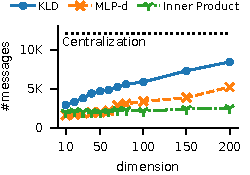
\includegraphics[width=0.47\columnwidth]
	    {figures/dimension_communication.pdf}
	}\hfill
	\subfloat[Impact of number of nodes $n$.]{
	    \label{fig:num_nodes_vs_communication}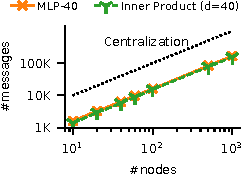
\includegraphics[width=0.47\columnwidth]
	    {figures/num_nodes_vs_communication.pdf}
	}
	\caption{
		Impact of dimension and the number of nodes on AutoMon's communication.
	}	
	\label{fig:dimension_impact}
\end{figure}


\subsection{Scalability: Dimensions, Nodes, Runtime}
\label{sec:scalability}

We use the KLD, Inner Product, and MLP-$d$ functions to study how data dimensionality affects the communication and runtime of AutoMon, as well as its ability to scale with the number of nodes.
For every function, we carry out multiple runs with input dimension $d \in [10,200]$.
As shown below, at high dimensions the bottleneck becomes the numerical optimization in full sync.
To compare the different functions and datasets, we set the number of nodes to $n=12$ and stop each run exactly 1000 rounds after the first sliding window is full,  resulting in a centralized cost of 1000 messages per node.
Runtimes are measured on an Intel i9-7900X at 3.3GHz with 64GB RAM, running Ubuntu 18.04 with MKL 2019 Update 3.


\betterparagraph{Dimensionality}
Prior work has shown that the size of the local vector $x$ can increase the number of messages needed to monitor a function~\cite{gabel:monitoring_least_squares}.
However, for AutoMon, the function itself is also a parameter, and we explore how their combination impacts communication.
Figure~\ref{sub_fig:dimension_communication} shows the total number of messages in each run for different functions and input dimensions.
We observe that AutoMon's scalability is highly dependent on which function is being monitored.
While communication increases with dimension for all functions, this increase is minimal for Inner Product, moderate for MLP-$d$, and more drastic for KLD.
Nevertheless, even for KLD, we observe that AutoMon remains better than centralization for up to 200 dimensions.


\betterparagraph{Number of Nodes}
More nodes means more communication, but this growth is contingent upon the distribution of the data between different nodes.
Figure~\ref{fig:num_nodes_vs_communication} illustrates how the number of messages grows with the number of AutoMon nodes for Inner Product ($d=40$) and MLP-40.
While the number of messages does increase with the number of nodes in the system, we observe that the same happens for Centralization, and that the ratio between Centralization and AutoMon is fixed.
In these synthetic datasets, the data of new nodes is similar to the data of existing nodes.
Therefore, the probability for violation of a single node does not change with the number of nodes, neither does the probability of resolving violations using lazy sync, which explains the fixed ratio.
We therefore conclude that the AutoMon technique does not limit the scalability of the system.
This limitation may emerge from the data itself.


\betterparagraph{Node Runtime}
AutoMon's node runtime should be low since it is targeting environments where the computational power of local data sources is low.
%
We measured the time a node takes to check a single data update, as well as the time it takes the node to complete different tasks during the data update process (figures omitted for lack of space).
The impact of the dimension on the average runtime is negligible, on average 1 millisecond or less for all functions and dimensionality.
The time to verify that the local vector is inside the safe zone is close to the time it takes to simply evaluate the original function on the local vector, ranging from 0.01 to 1 millisecond.
We therefore conclude that AutoMon node is suitable even for computationally limited edge devices.


\betterparagraph{Coordinator Runtime}
While AutoMon's coordinator may not be a resource-constrained edge device, the coordinator's runtime limits the data rate supported by AutoMon because nodes must wait for the coordinator to resolve violations.
This runtime is dominated by the full sync with ADCD-X, which requires solving a numerical optimization problem to find the extreme eigenvalues.
The lazy sync time is orders of magnitude smaller, as it only requires evaluating the local constraints.
%
For KLD and MLP-$d$, which use ADCD-X, the average time for the full sync increases with the dimension, ranging from 0.2 seconds ($d=10$) to 12 seconds ($d=200$).
For Inner Product, the coordinator uses ADCD-E, where eigendecomposition is done only once at initialization; full sync time is below 10 milliseconds for all dimensions.
(Figure omitted for lack of space.)







\subsection{Impact of Neighborhood Size Tuning}
\label{sec:eval-sub-domain-size}

To demonstrate the effectiveness of Algorithm~\ref{algo:sub_domain_tuning},
we show that 
\begin{enumerate*}
\item the $\hat{r}$ found by the algorithm is close to the true optimal neighborhood size $r^*$;
\item $r$ can have a large impact on AutoMon's communication;
\item no single fixed $r$ is optimal across different approximation error bounds $\epsilon$; and
\item the tuning procedure yields comparable performance to using the optimal $r^*$.
\end{enumerate*}


To evaluate Algorithm~\ref{algo:sub_domain_tuning} we used AutoMon with a range of approximation error bounds $\epsilon$ and neighborhood sizes $r$ to monitor the MLP-2 function, as well as the Rozenbrock function, defined as $f(x) = (1 - x_1)^2 + 100 \left(x_2 - x_1^2\right)^2$.
We chose this function because it is especially challenging for gradient-based numerical approaches (e.g., AutoMon or gradient descent), and because its Hessian is non-constant. To generate data, we draw entries $x_1,x_2$ from the normal distribution $\mathcal{N}(0, 0.2^2)$.
%
For each approximation error bound $\epsilon$, we find the optimal neighborhood size $r^*$ that obtains the smallest number of violations, as well as the recommended neighborhood size $\hat{r}$ found by the tuning procedure.
We repeated each experiment $5$ times, sampling a new dataset every run.

On average, the true optimal neighborhood size $r^*$ is close to the neighborhood size found by the tuning procedure $\hat{r}$ (figure omitted due to lack of space), especially given the significant effect of the randomness in the data.
The mean relative error of the tuning algorithm with respect to the optimal value is $8\%$ for Rozenbrock and $20\%$ for MLP-2.
On average, we find that $\hat{r}$ found by Algorithm~\ref{algo:sub_domain_tuning} is within 1.03 standard deviations of the optimal $r^*$ for both functions.
Rozenbrock is highly sensitive to small input changes by design.
Hence, the standard deviation for $\hat{r}$ is large while $r^*$ has a small range (as Figure~\ref{fig:neighborhood_impact_on_communication_error_bound_connection} shows).
Conversely, MLP-2 is less sensitive. 
It has a wider range of optimal $r^*$, while the tuning procedure tends to converge to same $\hat{r}$.


\begin{figure}
	\centering
	{\label{sub_fig:neighborhood_impact_on_communication_error_bound_connection}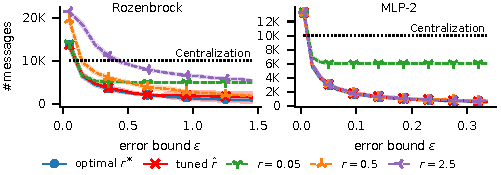
\includegraphics[width=1.0\columnwidth]{figures/neighborhood_impact_on_communication_error_bound_connection.pdf}}
	\caption{
		Mean number of messages for different approximation error bounds $\epsilon$, while using optimal neighborhood size $r^*$, tuned size $\hat{r}$, and fixed $r$ during monitoring.
		The standard deviation is small and barely visible (shaded area).
	}
	\label{fig:neighborhood_impact_on_communication_error_bound_connection}
\end{figure}


To evaluate the impact of $r$ on communication,
we run AutoMon over the sampled datasets, each with its optimal $r^*$ and the tuned $\hat{r}$, as well as three fixed neighborhood sizes $r \in \{0.05, 0.5, 2.5\}$.
Figure~\ref{fig:neighborhood_impact_on_communication_error_bound_connection} shows AutoMon's average communication for each approximation error bound $\epsilon$.
We make three observations.
First, using the wrong $r$ can substantially increase communication.
Second, no single $r$ is best across all $\epsilon$ and functions.
For example, for Rozenbrock the average increase in the number of messages when using $\hat{r}$  instead of $r^*$ is $33\%$, while for the fixed $r$ it grows by more than $100\%$.
For MLP-2, the difference between $r^*$ and $\hat{r}$ is $3.5\%$; however, for the best other fixed $r$ it is more than $7\%$.
The results for MLP-2 also suggest there is a range of neighborhood sizes that work well; however, this range is not known a-priori.
Third, and most crucial, we observe that using the $\hat{r}$ found by the tuning process results in a similar number of messages as using the optimal neighborhood  $r^{*}$.



\subsection{Impact of ADCD, Slack, and Lazy Sync} \label{sub_sec:rlv_and_lazy_sync}

We perform an ablation study to evaluate the contribution of different components of AutoMon.
Could we replace the ADCD local constraints with simply checking the global condition on local data $L \leq f(x) \leq U$, relying on the GM protocol to reduce communication?
As shown below, even for simple functions with only few nodes, this is not the case.


We demonstrate this using the function $f(x) = -x_1^2 + x_2^2$ with four nodes.
We simulate 1000 rounds with the local data for the four nodes initially the same, starting at $(x_1, x_2)=(0,0)$.
As the experiment progresses, local node data slowly drifts in different directions, which is common in distributed setting. Specifically, the local vectors move towards $(1,0)$, $(-1,0)$, $(1,1)$ and $(1,-1)$).
For two nodes, we also add outliers between rounds 650 and 700.


\begin{figure}
	\centering
	\subfloat[$f(x)=-x_1^2+x_2^2$.]{
	    \label{sub_fig:monitoring_stats_quadratic_inverse}
	    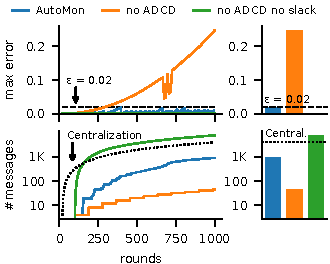
\includegraphics[width=0.65\columnwidth]{figures/monitoring_stats_quadratic_inverse.pdf}
	}
	\subfloat[MLP-2.]{
	    \label{sub_fig:monitoring_stats_barchart_mlp_2}
	    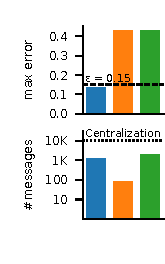
\includegraphics[width=0.32\columnwidth]{figures/monitoring_stats_barchart_mlp_2.pdf}
	}	
	\caption{
	    Impact of AutoMon features on approximation error (top) and cumulative communication (bottom) when monitoring $f(x)=-x_1^2+x_2^2$ (left) and MLP-2 (right); lower is better.
		ADCD and slack are both needed to achieve low error and low communication.
	}
	\label{fig:monitoring_stats}
\end{figure}


Figure~\ref{sub_fig:monitoring_stats_quadratic_inverse} shows the approximation error (top) and cumulative messages (bottom) of each algorithm over time. 
AutoMon maintains the desired approximation error using minimal communication, since the ADCD local constraints for $f$ are both correct and efficient.
Without ADCD, however, the monitoring suffers from missed violations: locally for every node $i$, $L \leq f(x^i) \leq U$, yet globally $L > f(\bar{x})$ or $f(\bar{x}) > U$.
This happens because lazy sync manages to balance the slack of different nodes, preventing the global sync from recomputing the reference point $x_0$.
The end result is unbounded and ever-increasing error, albeit with little communication.
We further removed slack and lazy sync, which gave us a basic GM protocol: similar to Algorithm~\ref{algo:protocol} but without ADCD.
This results in a low approximation error due to many full sync operations, but at the cost of more communication than would be used by a centralization approach (which would result in no error).

We repeated the experiment with the more complex MLP-2 function and present the results in Figure~\ref{sub_fig:monitoring_stats_barchart_mlp_2}.
Without ADCD, the approximation error grows to over twice the size of the bound.
Unlike before, removing the slack and lazy sync mechanism does not help since for MLP-2 it is even more likely that locally $L \leq f(x^i) \leq U$ while globally $L > f(\bar{x})$ or $f(\bar{x}) > U$.
In contrast, AutoMon maintains the desired approximation with low communication by synchronizing as needed.





\subsection{Validation on Real-World Deployment}
\label{sec:distributed-experiment}

Simulations let us compare algorithms while controlling important variables (such as $n$, $d$) in isolation from confounders (e.g., choice of network stack).
%
We now verify our simulation in Section~\ref{sub_sec:error_communication_tradeoff} through a series of geo-distributed experiments.
We conducted each run in our experiments on two Amazon ECS clusters~\cite{amazonecs}: one is located in us-west-2 region and is comprised of a single coordinator using 16 vCPUs and 32GB of memory on an Intel Xeon CPU at 3.4--3.9 GHz;
the other is located in us-east-2 and includes all nodes, each with 1 vCPU and 4GB of memory on an Intel Xeon CPU at 2.2--2.5GHz;
the average RTT was 56ms.
For messaging, we used ZeroMQ~\cite{zeromq}.
We set the time between data updates to 5 seconds for DNN and to 1 second for the other datasets.
We count the total bytes in the payload of AutoMon's messages, and use Nethogs~\cite{nethogs} to monitor the traffic volume of the coordinator process, which includes both payload and overheads such as ZeroMQ and packet headers.

\begin{figure}
	\centering
	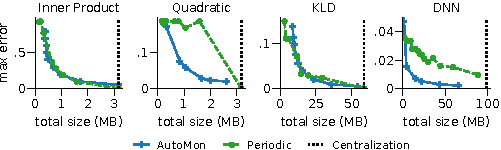
\includegraphics[width=1.0\columnwidth]{figures/max_error_vs_transfer_volume.pdf} 
	
	\vspace{3mm}
	
	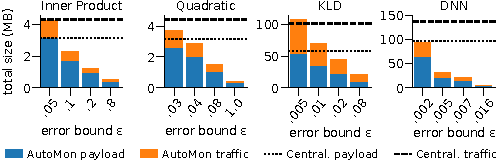
\includegraphics[width=1.0\columnwidth]{figures/communication_automon_vs_network.pdf}
	\caption{
	    Bandwidth usage in distributed experiments over public WAN.
	    Top: error-bandwidth tradeoff, with
	    X axis showing total size of message payload for each monitoring approach.
	    Bottom: AutoMon's total message payload size and measured 
	    network traffic for a range of $\epsilon$ values from the distributed experiments in Figure~\ref{fig:max_error_vs_transfer_volume}.
	    Horizontal lines depict centralization payload size and network traffic.
	}
	\label{fig:max_error_vs_transfer_volume}
	\label{fig:communication_automon_vs_network}
\end{figure}

\betterparagraph{Number of Messages}
Real-world communication matches our simulation, with a median difference of 0\% for the DNN function, less than 5.3\% for inner product and KLD, and 16.6\% for Quadratic (figure omitted).
Slight timing differences when nodes update their local data result in a small number of additional messages, as the coordinator requests the local vectors for nodes after they had already reported a local violation.

\betterparagraph{Error-Bandwidth Tradeoff}
The top of Figure~\ref{fig:max_error_vs_transfer_volume} shows the error as a function of total payload size.
The error-bandwidth tradeoff generally agrees with the error-communication tradeoff in Figure~\ref{fig:error_communication_tradeoff}.
The relative ranking of methods is also the same:
AutoMon's total payload size is lower than that of Periodic whenever AutoMon uses less messages than Periodic.

\betterparagraph{Network Traffic Consumed}
The bottom of Figure~\ref{fig:communication_automon_vs_network} shows AutoMon's total payload size (blue) and actual network usage (orange) for a range of $\epsilon$ values.
The dotted line is Centralization's payload size and the dashed line is its network traffic.
In most cases, except in the extreme cases for a very small $\epsilon$ value, AutoMon's usage is less than Centralization's payload.
It reduces data transfer volumes by up to 98\%, depending on the requested error bound $\epsilon$, and by 65\% on average across all tested functions and error bounds.
